\documentclass[stage]{tnreport}

\usepackage[utf8]{inputenc} 

\def\reportTitle{Mise en place d’un service de compilation/d’exécution isolé pour la plateforme PLM dédiée à l’apprentissage de la programmation} % Titre du mémoire
\def\reportLongTitle{Mise en place d’un service de compilation/d’exécution isolé pour la plateforme PLM dédiée à l’apprentissage de la programmation} % Titre plus long du mémoire

\def\reportAuthor{Tanguy GLOAGUEN}
\def\reportAuthorEmail{\email{tanguy.gloaguen@telecomnancy.eu}} % Courriel de l'élève

\def\reportSupervisor{Martin QUINSON, Gérald OSTER} % Prénom Nom de l'encadrant industriel

\def\reportCompany{LORIA} % Nom de l'entreprise d'accueil
\def\reportCompanyAddress{Campus Scientifique}  % Adresse de l'entreprise
\def\reportCompanyCity{54506, Nancy} % Adresse (cont.) de l'entreprise
\def\reportCompanyPhone{~} % Téléphone de l'entreprise
\def\reportCompanyLogoPath{figures/LORIA-logo.jpg} % Logo de l'entreprise

\def\place{Nancy} % Ville pour la signature pour l'engagement anti-plagiat
\def\date{\today} % Date pour la signature de l'engagement anti-plagiat

\def\reportProjectCustomer{}

\begin{document}

\maketitle
\pagenumbering{roman}

\insertAntiPlagiarismAgreement{GLOAGUEN, Tanguy}{31313847}

\cleardoublepage

\makesecondtitle

\section*{Remerciements}
\addcontentsline{toc}{chapter}{Remerciements}

{\em
Je tiens tout d'abord à remercier mes encadrants de stage, MM. Oster et Quinson, pour leur accueil au sein de leur équipe, leurs conseils et explications sur le système à étudier et le temps qu'ils ont accordé à l'étude des modèles proposés.

Je remercie également Matthieu Nicolas, qui m'a également encadré lors de ce stage, pour son aide précieuse sur les outils à utiliser, mais aussi pour son écoute et ses conseils quant aux méthodes de résolution des problèmes étudiés.

Enfin, je remercie mes collègues de bureau, MM. Bühler, Carpentier et Grguric, pour leurs aides sur la réalisation et pour l'ambiance agréable de travail.
}

\cleardoublepage

\renewcommand{\baselinestretch}{0.5}\normalsize
\tableofcontents
\renewcommand{\baselinestretch}{1.0}\normalsize
\cleardoublepage

\pagenumbering{arabic}
\setcounter{page}{1}

\chapter*{Introduction}

L'enseignement classique est celui généralement utilisé aujourd'hui, mais l'accés au public de l'informatique a permi de mettre en place des apprentissages plus automatisés : outils d'aide à l'enseignement, MOOC (cours en ligne) mais aussi logiciels d'apprentissage autonome.
C'est dans ce contexte que se place la Programmer's Learning Machine : depuis 2007, cette application permet de standardiser les enseignements de base en programmation ainsi que d'aider les enseignants à évaluer les progrès des élèves.
La PLM a pour but d'enseigner les bases de la programmation et de fournir aux éudiants les meilleurs outils possibles pour apprendre à coder.

En vue de moderniser le logiciel, il a été récemment proposé de transformer l'application PLM en un outil en ligne. Cette modification a entraîné des contraintes de sécurité, de puissance du matériel, de consommation mémoire et processeur des services et de mise à l'échelle supplémentaires qu'il a fallu résoudre.

L'objectif de ce stage était de proposer des solutions à ces contraintes, de les implémenter et de proposer des méthodes de déploiement.

Dans un premier temps, nous verrons le contexte du stage plus en détail : l'établissement d'accueil mais aussi la Programmer's Learning Machine en tant qu'application et qu'interface web.

Dans un second temps, nous verrons les objectifs du stage.

Puis, nous étudierons la réalisation de ces objectifs en tant que méthodologie, en tant qu'environnement et les résultats obtenus.

Enfin, nous ferons un bilan des résultats et une liste des améliorations prévues et possibles.

\cleardoublepage

\chapter{Présentation}

\section{Le LORIA}

Le Laboratoire Lorrain de Recherche en Informatique et ses Applications (abrégé LORIA) est une Unité Mixe de Recherche créé en 1997 par association entre le CNRS (Centre National de la Recherche Scientifique), l'UL (Université de Lorraine) et l'INRIA (Institut National de Recherche en Informatique et Automatique).

La mission principale du LORIA est la recherche fondamentale et appliquée dans le cadre des sciences informatiques. Elle accueille un total de 450 personnes\footnote{chiffres 2014, http://www.loria.fr/rapports-activite-2/rapport-dactivite-2014}, réparties en 27 équipes sur 5 dépatements :
\begin{description}
	\item[Algorithmique, calcul, image et géométrie] \hfill \\
		Ce département de 6 équipes, dirigé par Sylvain Lazard, s'intéresse principalement aux algorithmes tout en gardant une différence sur les applications selon les équipes.
	\item[Méthodes formelles] \hfill \\
		 Ce département de 6 équipes, dirigé par Dominique Méry, développe des contributions aux logiques et théories de preuves. C'est dans ce département que se trouve VERIDIS et le projet PLM.
	\item[Réseaux, systèmes et services] \hfill \\
		 Département de 3 équipes dirigé par Ye-Quiong Song, il s'intéresse principalement aux problèmes issus des systèmes distribués et parallèles.
	\item[Traitement des langues et des connaissances] \hfill \\
		 Ce département de 8 équipes dirigé par Bruno Guillaume porte sur l'étude des langues naturelles, des conaissances et des documents.
	\item[Systèmes complexes et intelligence artificielle] \hfill \\
		 Département de 5 équipes dirigé par Bernard Girau, il s'occupe des méthodes d'apprentissage, d'analyse et de prise de décision rendus possibles par les intelligenes artificielles.
\end{description}

\clearpage

\begin{figure}[h]
	\centering
		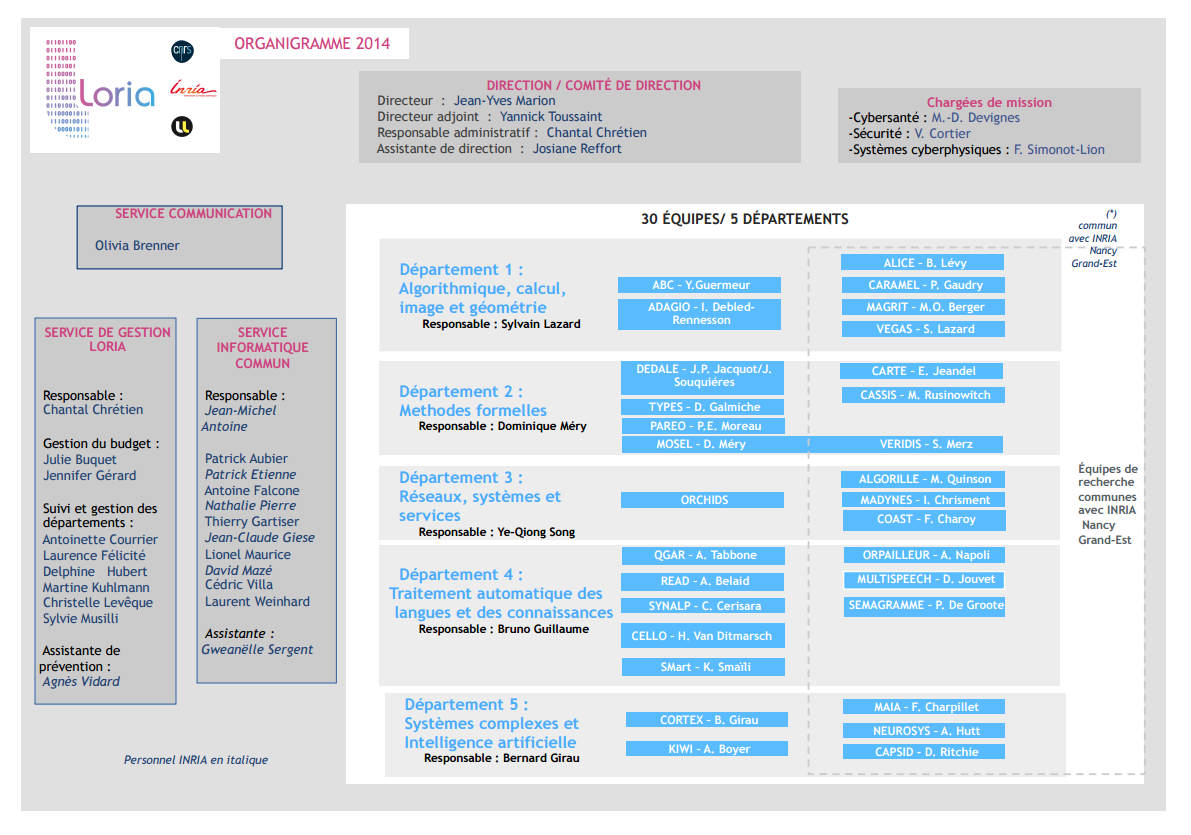
\includegraphics[width=0.9\textwidth]{figures/LORIA-organigramme}
	\caption{Organigramme du LORIA}
	\label{fig:organigramme}
\end{figure}

En tant qu'UMR, le LORIA possède sa propre administration. Un organigramme du LORIA est dispobible en \ref{fig:organigramme}, présentant la structure interne. On y remarque que même si les différentes entités administratives sont bien définies, il n'y a pas de hiérarchie directe entre elles.


\section{La "Programmer's Learning Machine"}

Le projet "Programmer's Learning Machine" (abrégé PLM) est un projet commencé en 2007 par Martin Quinson et Gérald Oster.

Ce projet a pour but de fournir aux étudiants en informatique une plateforme d'initiation aux concepts de programmation basiques et avancés ainsi qu'un outil d'analyse et d'aide à la médiation pour l'enseignant.
La PLM est utilisée depuis à Telecom Nancy, et sert en première année à aider à la formation des nouveaux étudiants. Elle possède pour le moment plus de 200 exercices distincts portant sur divers sujet allant de l'introduction aux concepts de programmation à la récursivité ou aux tris.

\subsection{La PLM en tant qu'application lourde}

Dans sa forme originelle, la PLM était une application Java lourde écrite en Swing. L'utilisateur lançait le programme sur son ordinateur et obtenait des résultats. L'application lourde est aujourd'hui en version 2.6 et approche de la version 2.7.

La PLM est constituée d'exercices, regroupés en leçons et étendus sur différents univers : buggles, turmites, tortues mais aussi listes ou même simple tests sans interface particulière. Chaque exercice propose donc un scénario dans ces univers, présentant un nouveau concept à l'utilisateur.
Celui-ci doit alors trouver quel code permet de résoudre l'exercice en s'aidant de la démonstration, du texte de mission et de l'API\footnote{API : Application Program Interface, ensemble des commandes spécifiques au programme. Ici, il s'agit des commandes de l'univers.} du monde.
\begin{figure}[h]
	\centering
		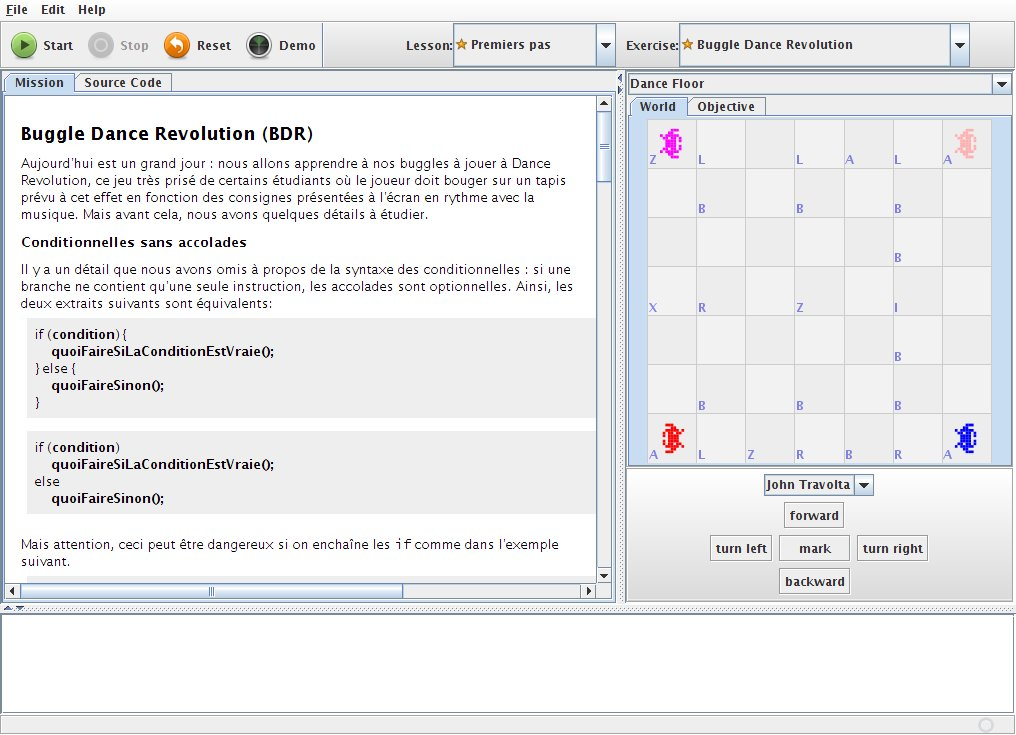
\includegraphics[width=0.9\textwidth]{figures/PLM-exercice1}
	\caption{Exemple d'exercice : Buggle Dance Revolution, portant sur la lecture d'informations et le pattern matching.}
	\label{fig:plmEx1}
\end{figure}

La PLM a été la cible de différents projets au cours du temps, de manière à ajouter des fonctionnalités : langage C, nouveaux exercices et nouvelles leçons et plus récemment aide spécifique à l'utilisateur et aux enseignants.

\subsection{Portage web de la PLM}

En plus des améliorations apportées à la PLM elle-même, il est question depuis décembre 2014 d'un portage AngularJS de l'application. Ce projet, nommé WebPLM, est principalement géré par Matthieu Nicolas.
La nouvelle architecture proposée est une interface client utilisant angular.js reliée via une WebSocket à un serveur web tournant sous Play Framework.

De cette manière, il serait en fait possible de centraliser les informations (ce qui permettrait un partage plus facile des améliorations) mais aussi pour permettre à terme de l'intégrer aux MOOC de programmation.
\begin{figure}[h]
	\centering
		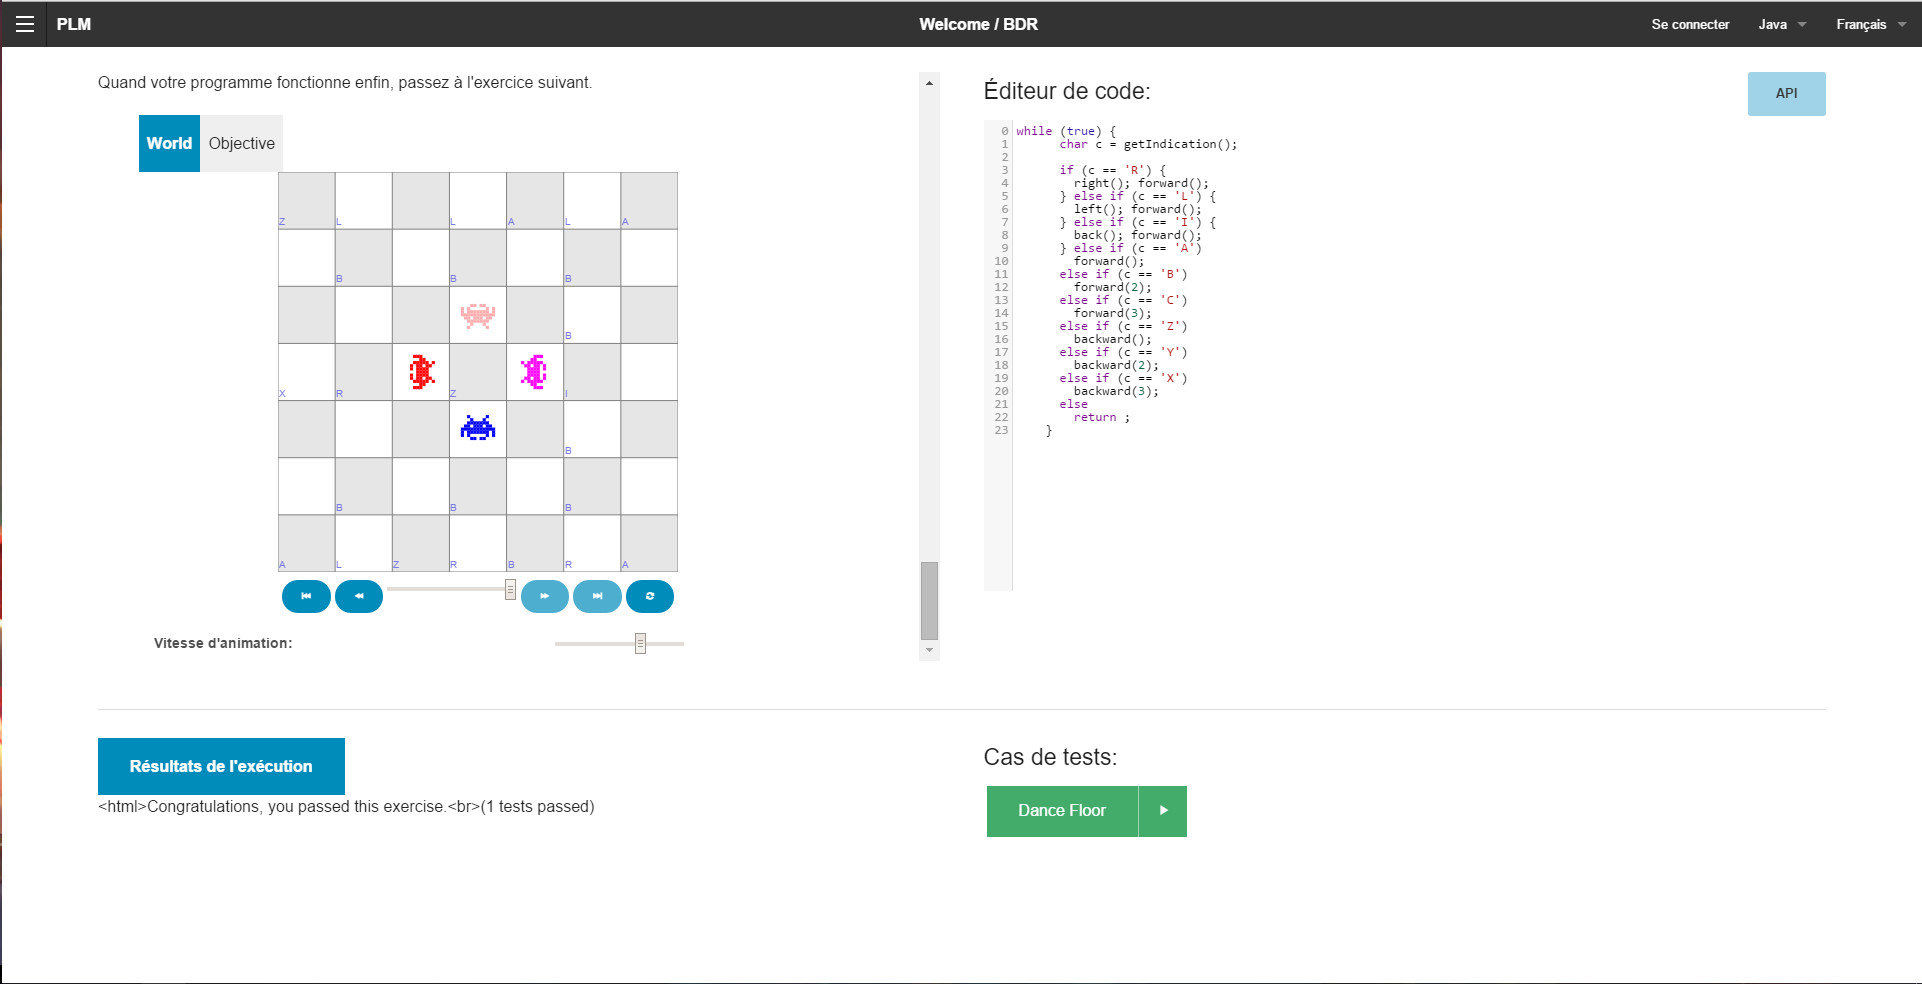
\includegraphics[width=0.9\textwidth]{figures/WebPLM-exercice1}
	\caption{Apparence de WebPLM, portage web de la PLM.}
	\label{fig:wplmEx1}
\end{figure}

Le portage web de PLM est aujourd'hui à un état utilisable, la plupart des exercices sont disponibles et les rares problèmes restants sont plus de l'ordre du confort visuel (problèmes d'affichage) ou de l'ordre de données non mises à jour.

\cleardoublepage

\chapter{Problématique du stage}

\section{Contexte du stage}

Le portage web entamé récemment portait principalement sur l'interface client et l'utilisation de PLM, sans se soucier des problèmes de performance ou de sécurité.
Le projet ayant aujourd'hui atteint un niveau ou son déploiement est envisageable, il est nécessaire d'adresser ces deux problèmes.

Pour palier à cela, MM. Quinson, Oster et Nicolas ont envisagé de séparer les deux composantes principales de la PLM : l'environnement d'exécution des exercices et l'environnement d'évolution de l'élève.
Cette solution permettrait donc d'isoler l'exécution dans des environnements contrôlés et dont la performance peut être mise à l'échelle.

Cependant, la PLM n'a pas été prévue pour séparer ces deux fonctions, il fallait donc comprendre le code d'origine et mettre en place une stratégie pour le séparer.

\section{Objectifs du stage}

Ce stage avait donc pour objectif de séparer les composantes de compilation/exécution de code élève et de gestion du progrès de l'élève.

Les objectifs du stage ont donc été de :
\begin{itemize}
	\item Identifier les composantes d'exécution et de gestion de l'élève dans la PLM.
	\item Créer un outil d'exécution de code
	\item Utiliser cet outil lors de la demande d'exécution de code
	\item Rendre l'outil sécurisé et distribuable.
	\item Améliorer la PLM pour retirer les composantes inutiles
\end{itemize}

Les pistes proposées par les encadrants de stages étaient de :
\begin{itemize}
	\item Utiliser une queue de message pour stocker les informations de compilation
	\item Utiliser la technologie Docker pour rendre le système distribuable.
	\item Utiliser Docker + un SecurityManager pour sécuriser l'environnement d'exécution.
\end{itemize}

\cleardoublepage

\chapter{Réalisation}
\section{Environnement de réalisation}

La réalisation s'est principalement faite sur un environnement de développement Windows et un environnement d'exécution Linux.

Les technologies utilisées étaient :
\begin{description}
	\item{Docker} \hfill \\
		Docker est une technologie de gestion d'applications distribuées. Le principe est de créer des images de machines virtuelles (appelées images docker) qui, une fois lancées, sont directement utilisables avec tous logiciels lancés. \\
		Une telle technologie a pour effet de rendre presque trivial la mise en production et la mise à l'échelle des environnements.
	\item{RabbitMQ} \hfill \\
		Rabbit MQ est un gestionnaire de queue de message. Une queue de message est un  système permettant de stocker temporairement des données par "bloc". On peut se connecter à cette queue de message pour y déposer des blocs ou en demander un. \\
		L'idée est que les clients ne s'intéressent pas à qui traite les mesages, juste à ce qu'il soit traité.
	\item{Play Framework} \hfill \\
		Play Framework est une application de déploiement de serveur web. Il permet d'installer rapidement un environnement web basé sur une JVM (java ou scala). C'est le système choisi pour développer la version web de la PLM.
\end{description}

En plus de ces technologies, il était nécessaire de créer le modèle de l'application. Il a donc été nécessaire d'appliquer différents designs patterns.

\section{Méthode de réalisation}

\subsection{Modèle global envisagé}

Le modèle de WebPLM au début du stage était assez proche de celui de PLM. En effet, WebPLM "contenait" dans son intégralité Game, le composant principal de PLM. On obtenait donc les figures \ref{fig:plmUP1} et \ref{fig:wplmUP1} suivantes :
\begin{figure}[h]
	\centering
		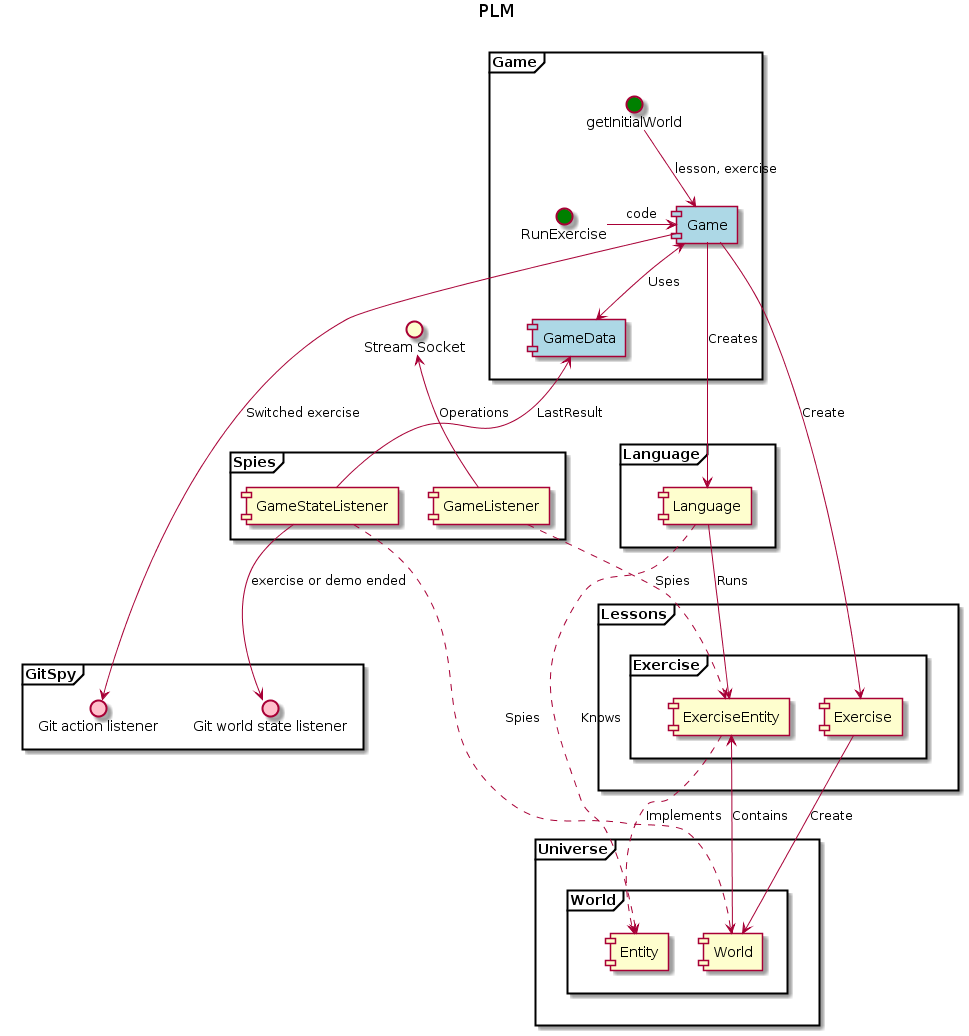
\includegraphics[width=0.5\textwidth]{figures/PLM-uml-cp1}
	\caption{Représentation complète de PLM à son exécution}
	\label{fig:plmUP1}
\end{figure}
\begin{figure}[h]
	\centering
		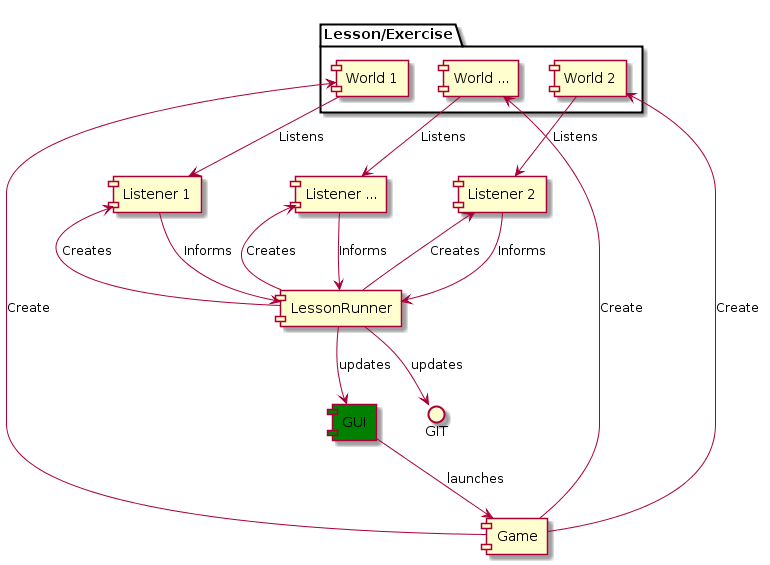
\includegraphics[width=0.7\textwidth]{figures/WebPLM-uml-cp1}
	\caption{Représentation simplifiée de WebPLM au début du stage}
	\label{fig:wplmUP1}
\end{figure}

Le but de l'amélioration est de séparer les appels de compilation du serveur. Pour commencer, la modélisation du problème en diagramme de séquence a été réalisée (fig \ref{fig:wplmUS1}).
\begin{figure}[h]
	\centering
		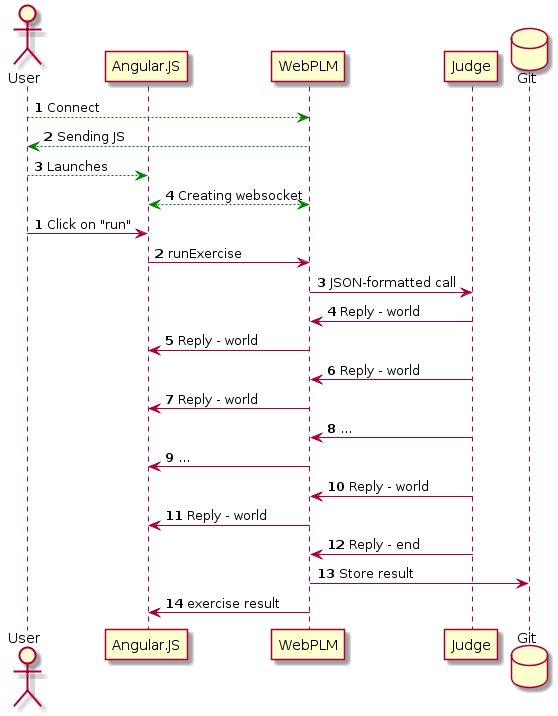
\includegraphics[width=0.4\textwidth]{figures/WebPLM-uml-Seq1}
	\caption{Diagramme de séquence du problème. En vert est l'étape de connexion, déjà créée dans WebPLM au moment du stage}
	\label{fig:wplmUS1}
\end{figure}

Il a été envisagé dans un premier temps de remplacer les appels de compilation par des appels RMI.
Cependant, la technologie RMI de Java n'était pas prévue pour récupérer plus d'un résultat, ce qui posait problème vu que le juge est supposé informer des changement d'états du monde au fur et à mesure de son exécution.

Le modèle envisagé a donc été dans un second temps un gestionnaire de queue de messages, RabbitMQ. Il permettait en effet de distribuer la charge de façon automatique mais aussi de créer automatiquement un protocole de retour dans des queues de messages indépendantes.

\subsection{Création des juges}

Les juges sont de simples conteneurs de la version de PLM déjà présente dans WebPLM. Cependant, ils possèdent une interface leur permettant de communiquer avec une queue de message.

La création des juges permit également de mettre en place des tests automatiques de compilation, nécessaire lorsque WebPLM n'était pas encore à jour. Les tests sont toujours en place dans les juges et permettent encore de tester la viabilité des changements de code sur des exercices simples et plus complexes.

Cette étape a duré approximativement deux jours, terminée le 26-06.

\subsection{Utilisation des juges}

Dans un second temps, il était nécessaire de refabriquer l'étape de compilation de WebPLM. Pour cela, il a fallu dans un premier temps écrire la structure d'appel et de récupération depuis la queue de message, puis de reformater le code de manière à le rendre utilisable.

\subsubsection{Système de base}
Tout d'abord, il a fallu écrire un système de base permettant à WebPLM d'utiliser la message queue pour gérer les appels de compilation et d'en rcupérer les résultats pour les transmettre au client.

L'étape d'écriture du code a pris environ 3 jours, terminée le 01-07. A ce moment, WebPLM utilisait déjà des juges parallélisables pour la compilation.

\subsubsection{Stockage du résultat}
Il fallait ensuite réécrire les appels au gestionnaire GIT de manière à enregistrer la progression de l'élève ainsi que son code. Il a été nécessaire d'extraire le gestionnaire du Game toujours présent dans WebPLM et de l'utiliser à partir de là.

Cette étape a duré deux autres jours, terminée le 03-07.

\subsubsection{Analyses de performances, limites d'exécution, arrêt automatique}
Enfin, il a fallu tester les performances et adapter le résultat en conséquence.

La première version avait d'énormes problèmes de performance. Cela était dû au fait que la queue de messages contenait un message par opération du monde, message générés en parallèle qui plus est.
J'ai donc mis en place un accumulateur au niveau des listeners (cf figure \ref{fig:wplmUP1}) pour n'envoyer qu'une opération toutes les 500ms. Cela a résolu le problème de performance de base.

Il y avait également un problème de stabilité lors de compilations se terminant en boucle infinie. Pour gérer cela, il a été mis en place un système de sémaphore avec tentative d'acquisition pendant X secondes (X vallait 30s, puis 15, puis 10 au fur et à mesure du projet), sémaphore réveillée par les listeners lors de la fin d'exécution.

Le résultat final était donc une version de PLM stable, décrite en figure \ref{fig:wplmUP2}.
\begin{figure}[h]
	\centering
		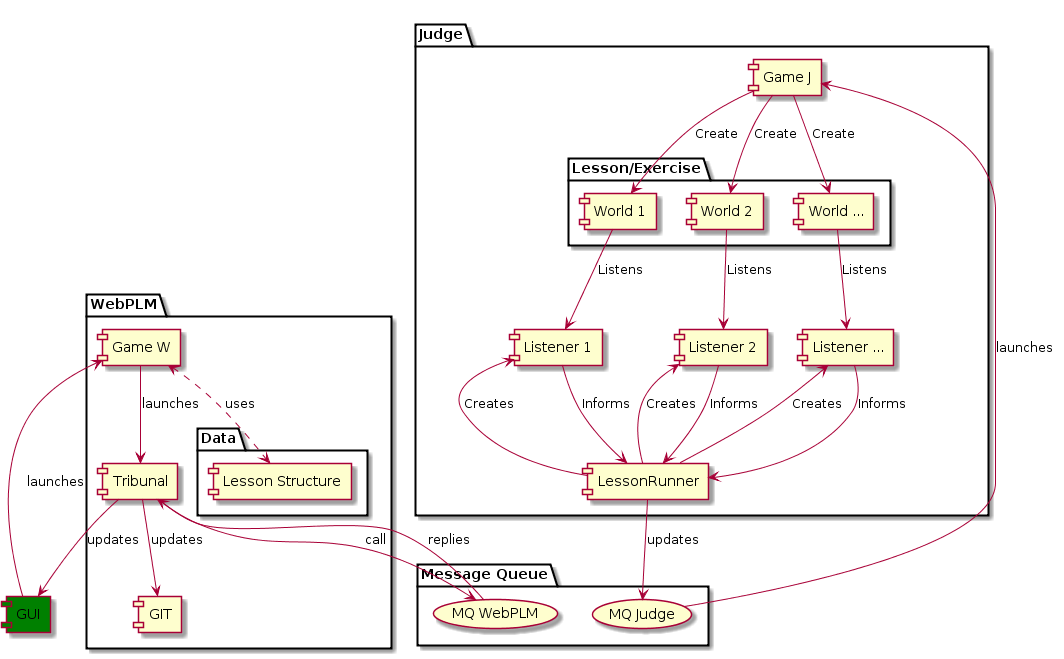
\includegraphics[width=0.7\textwidth]{figures/WebPLM-uml-cp2}
	\caption{Structure simplifiée de WebPLM et juges à la fin de l'étape de création des juges.}
	\label{fig:wplmUP2}
\end{figure}

\subsection{Etude d'un mode débug}

Pendant les semaines suivantes du stage, il a été question d'un mode "débug" de PLM. Ce mode débug devait permettre aux élèves d'avoir un aperçu de l'évolution de leurs variables et au système d'enseignement de détecter des schémas plus précis où l'élève resterait bloqué.

Différentes solutions ont été étudiées au cours du stage, en particulier la librairie JDI de Java pour détecter les modifications sur l'autre machine. Cependant, ce projet n'a jamais eu la priorité qu'il aurait fallu pour le mener à terme.

\subsection{Utilisation de Docker}

Après avoir modifié WebPLM pour se comporter en deux parties, il a été nécessaire d'adapter ces deux parties pour qu'elles puissent être utilisées dans des containers Docker.

Les principaux défis de cette étape n'ont pas été la réalisation elle-même mais la compréhension des différents problèmes rencontrés.

\begin{description}
	\item{Interaction entre Docker et Maven} \hfill \\
		Docker et Maven sont deux outils ayant des propriétés similaires : la centralisation des données en vue d'une utilisation déployable facilement. Le principal souci rencontré est lors de la génération des images Docker, Maven devant télécharger à chaque fois l'intégralité des composants. Le résultat était une compilation a réussite aléatoire.
	\item{Déploiement de RabbitMQ et utilisations de variables internes} \hfill \\
		Les différents composants de WebPLm avaient tous besoin d'un outil commun : la conaissance de l'adresse de la Message Queue. Il a fallu modifier WebPLM et les juges de manière à pouvoir récupérer ces informations automatiquement.
\end{description}

Cette étape aura duré du 09/07 au 16/07.

\subsection{Documentation du code existant}

Une phase de documentation et de refactoring a alors pris place. Maintenant que tous les composants étaient mis en place, il était possible de refabriquer les structures de données de manière à les adapter au mieux aux tâches qu'elles devaient réoudre.
Une javadoc des ajouts déjà effectués à été également réalisée de manière à rendre plus facile toute modification subséquente du code.

Cette étape s'est étendue sur les 20 et 21 juillet.

\subsection{Ajout d'opérations de logging}

Une étape de l'amélioration du projet WebPLM a été de rajouter l'affichage du canal de sortie standard sur l'écran de l'utilisateur. Pour cela, il a fallu capturer toutes les données de sortie standard et les rediriger en tant qu'opérations vers l'utilisateur. Il a également fallu recréer un canal spécifque permettant aux logs de l'application de tout de même apparaître sur la sortie standard.

Cette étape a pris place les 22/07 et 23/07.

\subsection{Standardisation des données}

Un problème assez particulier nous est apparu. Pour certains mondes, le code de résolution était entré et un juge validait le résultat, cependant l'affichage sur la WebPLM paraissait faux.

Il s'avère que la génération de certains mondes était aléatoire, ce qui provoquait une discordance entre les actions calculées à partir du monde du juge et celles appliquées sur le monde affiché. Il a donc fallu standardiser les mondes.

Pour cela, il a été appliqué une méthode simple : les fonctions aléatoires ont vu leur "seed" se faire fixer au même nombre. Selon la Javadoc, les résultats sont donc maintenant strictement identiques quelque sit le système utilisé.

Cela a été effectué le 24/07.

\subsection{Pré-génération des données}

En vue du passage a une version de WebPLM (côté serveur) sans la composante PLM, il fallait générer les données nécessaires (structures des execices, état initial des mondes, démonstrations) et les stocker de façon statique avant de pouvoir juste supprimer Game.

Pour arriver à ce résultat, il a fallu modifier un juge pour lui faire parcourir tous les exercices et, pour chacun, générer la démonstration et l'état initial.

Cette étape a été effectuée du 27/07 au 05/08

\subsection{Nettoyage de la PLM}

La dernière étape de ce stage a été de tenter de retirer PLM (en particulier Game) de WebPLM. Pour cela, il fallait étudier les différentes composantes utiles de PLM, les réécrire au mieux pour Play Framework (en Scala) et résoudre le diférents problèmes de taille mémoire et de concurrence qui aparaissaient.

Au début de cette étape, la structure de PLM était celle présentée en figure \ref{fig:wplmUP3}.
\begin{figure}[h]
	\centering
		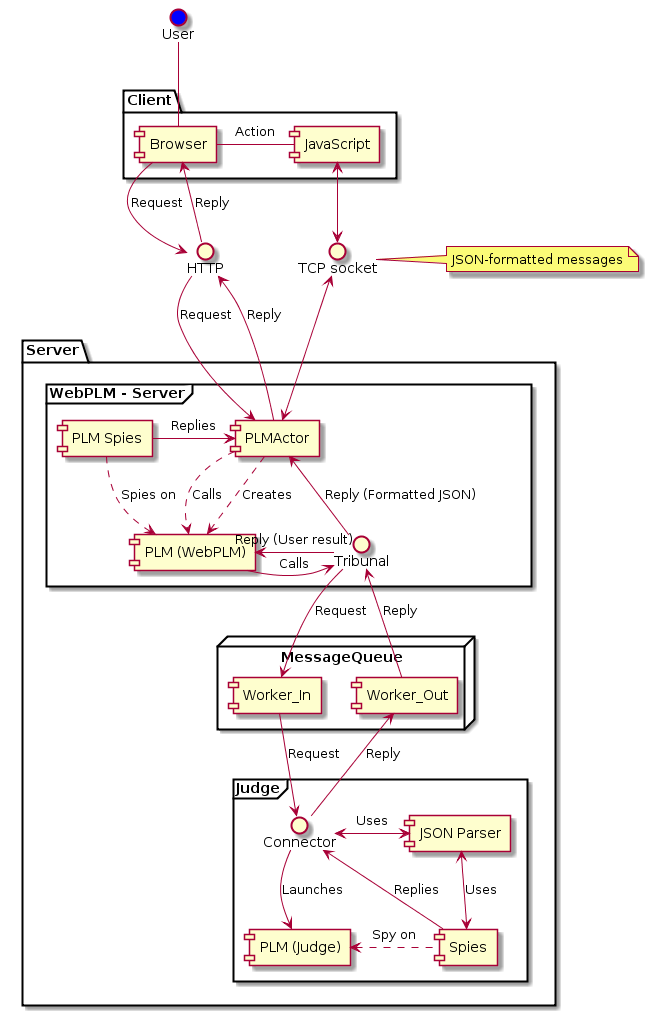
\includegraphics[width=0.5\textwidth]{figures/WebPLM-uml-cp3}
	\caption{Structure de WebPLM au début du nettoyage}
	\label{fig:wplmUP3}
\end{figure}

Le but était d'obtenir une structure telle que celle en \ref{fig:wplmUP4}.

\begin{figure}[h]
	\centering
		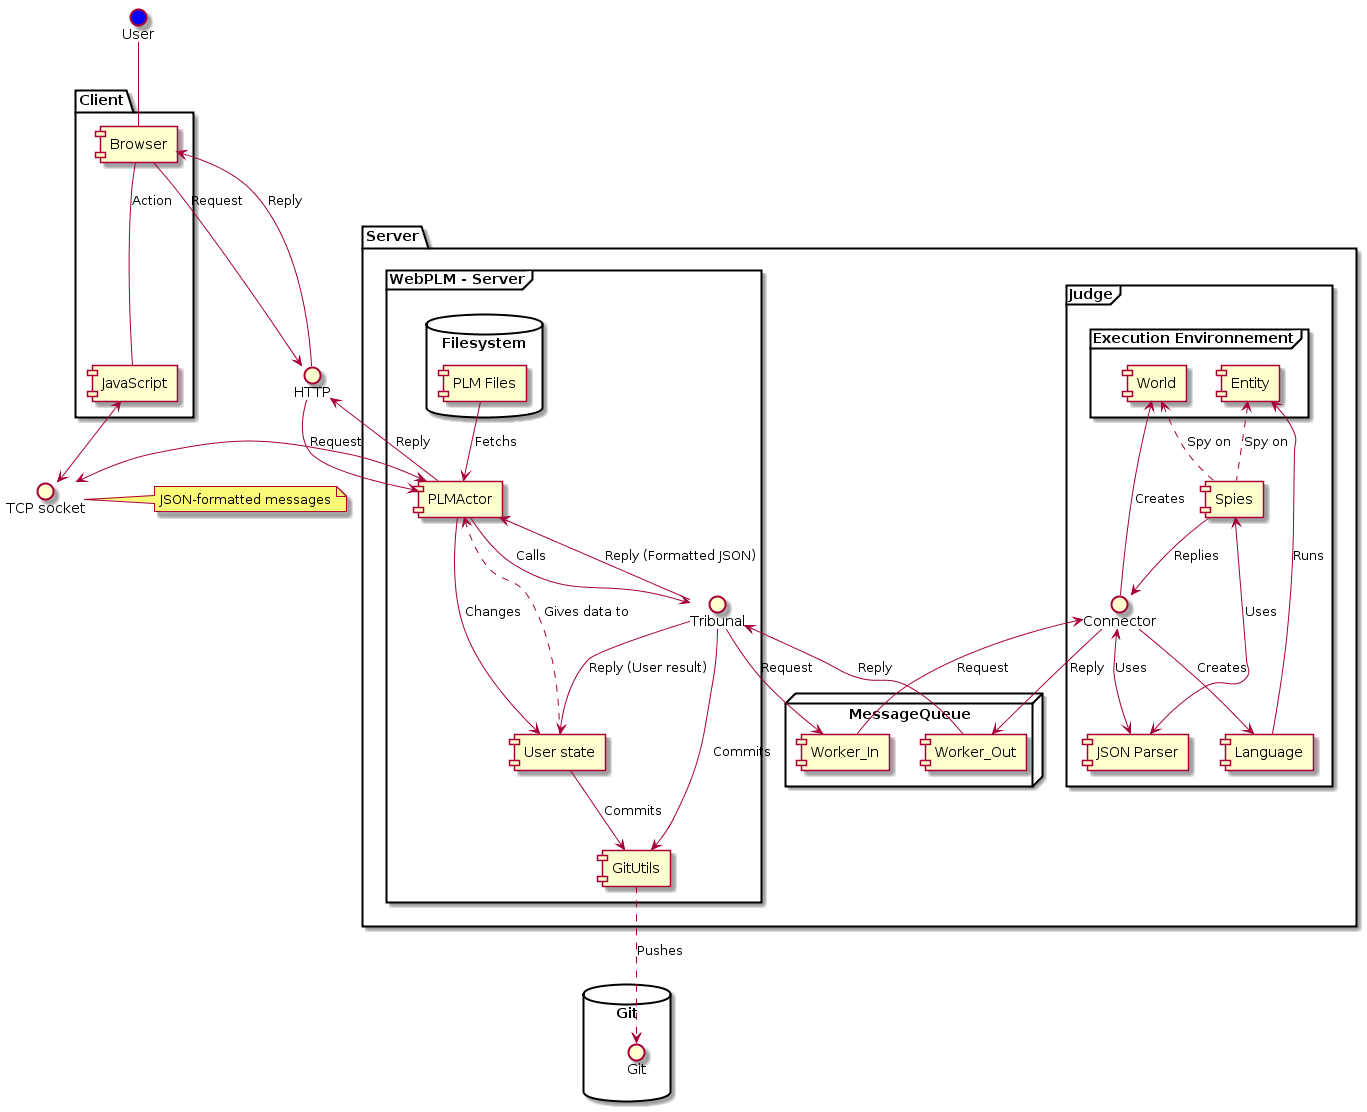
\includegraphics[width=0.9\textwidth]{figures/WebPLM-uml-cp4}
	\caption{Structure finale idéale de WebPLM.}
	\label{fig:wplmUP4}
\end{figure}

Les principales étapes de ce nettoyage ont été de retirer la composante de lecure de données, les missions (textes d'informations sur les exercices) et les APIs (textes d'informations sur les mondes), la composante de localisation ainsi que celle de gestion du langage de programmation. Il a fallu également convertir les fonctions de génération en fonction de lecture ou d'exposition : les démonstrations sont par exemple pré-générées et exposées en tant que fichiers par le serveur et c'est le client qui va les chercher pour les afficher, ce qui améliore énormément les performances du serveur.

Cependant, il reste un grand nombre de fonctions non converties : gestion du changement de leçon, d'exercice et de langue (naturelle/programmation), sauvegarde des données sur le gestionnaire GIT.

Cette tâche, commencée le 06/08, continue encore aujourd'hui.

\subsection{Mise en place d'un Security Manager}

Vers la fin de la période, nous nous sommes rendu compte que de nombreuses failels de sécurité que Docker était censé résoudre ne l'étaient en fait pas : accès à l'internet depuis un container, surcharge du processeur et surcharge du disque dur.

Pour résoudre certains de ces problèmes, nous avons utilisé un outil rendu disponible par Java, le Security Manager. Il permet de limiter les actions possibles pour chaque composante de l'application.

Nous avons donc limité les actions dispoibles à l'utilisateur, en lui interdisant toute communication avec l'extérieur du programme. Il restait tout de même plusieurs problèmes potentiels mais le résultat est qu'aucun de ces problèmes ne risque de briser la sécurité du système.

\section{Résultats obtenus}

\subsection{Modèle final}

Le modèle final de WebPLM est donc celui présenté en \ref{fig:wplmUP5}
\begin{figure}[h]
	\centering
		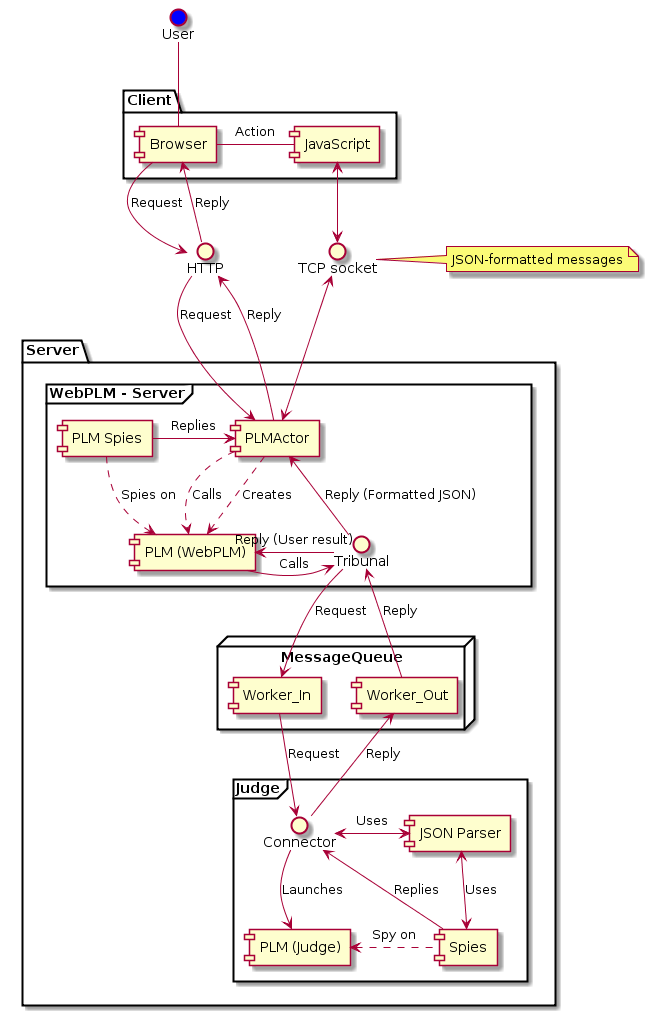
\includegraphics[width=0.7\textwidth]{figures/WebPLM-uml-cp3}
	\caption{Structure de WebPLM a la fin du stage.}
	\label{fig:wplmUP5}
\end{figure}

C'est effectivement la même structure qu'avant le nettoyage, a raison : au moment de l'écriture de ce rapport, l'opération de séparation des composants de Game n'est pas terminée et ne le sera probablement pas avant la fin du stage.

 \subsection{Apports}

Cependant, un certain nombre d'apports ont été faits à PLM au cours de ce stage.

Dans un premier temps, l'objectif principal de séparér composantes d'exécution et de gestion est accompli.

Il a été également rajouté des fonctons auxiliaires utiles : gestion de la sortie d'affichage standard, suppression des composantes aléatoires des exercices.

De gros progrès ont été également apportés sur l'étape de retrait de PLM depuis WebPLM.

Enfin, un travail de défrichage a été fait sur le mode débug.

\cleardoublepage 

\chapter{Résultats}

\section{Bilan}

Les réalisations lors de ce stage ont été conformes 

\section{Améliorations prévues}

\section {Améliorations possibles}

\cleardoublepage
\thispagestyle{empty}

\section*{Résumé}
\addcontentsline{toc}{chapter}{Résumé}

{\bf Mots-clés :}


\section*{Abstract}
\addcontentsline{toc}{chapter}{Abstract}

{\bf Keywords :}


\end{document}
